%% Run LaTeX on this file several times to get Table of Contents,
%% cross-references, and citations.

\documentclass[11pt]{book}
\usepackage{gvv}
\usepackage{gvv-book-bkup}
%\usepackage{Wiley-AuthoringTemplate}
\usepackage[sectionbib,authoryear]{natbib}% for name-date citation comment the below line
%\usepackage[sectionbib,numbers]{natbib}% for numbered citation comment the above line

%%********************************************************************%%
%%       How many levels of section head would you like numbered?     %%
%% 0= no section numbers, 1= section, 2= subsection, 3= subsubsection %%
\setcounter{secnumdepth}{3}
%%********************************************************************%%
%%**********************************************************************%%
%%     How many levels of section head would you like to appear in the  %%
%%				Table of Contents?			%%
%% 0= chapter, 1= section, 2= subsection, 3= subsubsection titles.	%%
\setcounter{tocdepth}{2}
%%**********************************************************************%%

%\includeonly{ch01}
\makeindex

\begin{document}

\frontmatter
%%%%%%%%%%%%%%%%%%%%%%%%%%%%%%%%%%%%%%%%%%%%%%%%%%%%%%%%%%%%%%%%
%% Title Pages
%% Wiley will provide title and copyright page, but you can make
%% your own titlepages if you'd like anyway
%% Setting up title pages, type in the appropriate names here:

\booktitle{CBSE Math}

\subtitle{Made Simple}

\AuAff{G. V. V. Sharma}


%% \\ will start a new line.
%% You may add \affil{} for affiliation, ie,
%\authors{Robert M. Groves\\
%\affil{Universitat de les Illes Balears}
%Floyd J. Fowler, Jr.\\
%\affil{University of New Mexico}
%}

%% Print Half Title and Title Page:
%\halftitlepage
\titlepage

%%%%%%%%%%%%%%%%%%%%%%%%%%%%%%%%%%%%%%%%%%%%%%%%%%%%%%%%%%%%%%%%
%% Copyright Page

\begin{copyrightpage}{2023}
%Title, etc
\end{copyrightpage}

% Note, you must use \ to start indented lines, ie,
% 
% \begin{copyrightpage}{2004}
% Survey Methodology / Robert M. Groves . . . [et al.].
% \       p. cm.---(Wiley series in survey methodology)
% \    ``Wiley-Interscience."
% \    Includes bibliographical references and index.
% \    ISBN 0-471-48348-6 (pbk.)
% \    1. Surveys---Methodology.  2. Social 
% \  sciences---Research---Statistical methods.  I. Groves, Robert M.  II. %
% Series.\\

% HA31.2.S873 2004
% 001.4'33---dc22                                             2004044064
% \end{copyrightpage}

%%%%%%%%%%%%%%%%%%%%%%%%%%%%%%%%%%%%%%%%%%%%%%%%%%%%%%%%%%%%%%%%
%% Only Dedication (optional) 

%\dedication{To my parents}

\tableofcontents

%\listoffigures %optional
%\listoftables  %optional

%% or Contributor Page for edited books
%% before \tableofcontents

%%%%%%%%%%%%%%%%%%%%%%%%%%%%%%%%%%%%%%%%%%%%%%%%%%%%%%%%%%%%%%%%
%  Contributors Page for Edited Book
%%%%%%%%%%%%%%%%%%%%%%%%%%%%%%%%%%%%%%%%%%%%%%%%%%%%%%%%%%%%%%%%

% If your book has chapters written by different authors,
% you'll need a Contributors page.

% Use \begin{contributors}...\end{contributors} and
% then enter each author with the \name{} command, followed
% by the affiliation information.

% \begin{contributors}
% \name{Masayki Abe,} Fujitsu Laboratories Ltd., Fujitsu Limited, Atsugi, Japan
%
% \name{L. A. Akers,} Center for Solid State Electronics Research, Arizona State University, Tempe, Arizona
%
% \name{G. H. Bernstein,} Department of Electrical and Computer Engineering, University of Notre Dame, Notre Dame, South Bend, Indiana; formerly of
% Center for Solid State Electronics Research, Arizona
% State University, Tempe, Arizona 
% \end{contributors}

%%%%%%%%%%%%%%%%%%%%%%%%%%%%%%%%%%%%%%%%%%%%%%%%%%%%%%%%%%%%%%%%
% Optional Foreword:

%\begin{foreword}
%\lipsum[1-2]
%\end{foreword}

%%%%%%%%%%%%%%%%%%%%%%%%%%%%%%%%%%%%%%%%%%%%%%%%%%%%%%%%%%%%%%%%
% Optional Preface:

%\begin{preface}
%\lipsum[1-1]
%\prefaceauthor{}
%\where{place\\
% date}
%\end{preface}

% ie,
% \begin{preface}
% This is an example preface.
% \prefaceauthor{R. K. Watts}
% \where{Durham, North Carolina\\
% September, 2004}

%%%%%%%%%%%%%%%%%%%%%%%%%%%%%%%%%%%%%%%%%%%%%%%%%%%%%%%%%%%%%%%%
% Optional Acknowledgments:

%\acknowledgments
%\lipsum[1-2]
%\authorinitials{I. R. S.}  

%%%%%%%%%%%%%%%%%%%%%%%%%%%%%%%%
%% Glossary Type of Environment:

% \begin{glossary}
% \term{<term>}{<description>}
% \end{glossary}

%%%%%%%%%%%%%%%%%%%%%%%%%%%%%%%%
%\begin{acronyms}
%\acro{ASTA}{Arrivals See Time Averages}
%\acro{BHCA}{Busy Hour Call Attempts}
%\acro{BR}{Bandwidth Reservation}
%\acro{b.u.}{bandwidth unit(s)}
%\acro{CAC}{Call / Connection Admission Control}
%\acro{CBP}{Call Blocking Probability(-ies)}
%\acro{CCS}{Centum Call Seconds}
%\acro{CDTM}{Connection Dependent Threshold Model}
%\acro{CS}{Complete Sharing}
%\acro{DiffServ}{Differentiated Services}
%\acro{EMLM}{Erlang Multirate Loss Model}
%\acro{erl}{The Erlang unit of traffic-load}
%\acro{FIFO}{First in - First out}
%\acro{GB}{Global balance}
%\acro{GoS}{Grade of Service}
%\acro{ICT}{Information and Communication Technology}
%\acro{IntServ}{Integrated Services}
%\acro{IP}{Internet Protocol}
%\acro{ITU-T}{International Telecommunication Unit -- Standardization sector}
%\acro{LB}{Local balance}
%\acro{LHS}{Left hand side}
%\acro{LIFO}{Last in - First out}
%\acro{MMPP}{Markov Modulated Poisson Process}
%\acro{MPLS}{Multiple Protocol Labeling Switching}
%\acro{MRM}{Multi-Retry Model}
%\acro{MTM}{Multi-Threshold Model}
%\acro{PASTA}{Poisson Arrivals See Time Averages}
%\acro{PDF}{Probability Distribution Function}
%\acro{pdf}{probability density function}
%\acro{PFS}{Product Form Solution}
%\acro{QoS}{Quality of Service}
%\acro{r.v.}{random variable(s)}
%\acro{RED}{random early detection}
%\acro{RHS}{Right hand side}
%\acro{RLA}{Reduced Load Approximation}
%\acro{SIRO}{service in random order}
%\acro{SRM}{Single-Retry Model}
%\acro{STM}{Single-Threshold Model}
%\acro{TCP}{Transport Control Protocol}
%\acro{TH}{Threshold(s)}
%\acro{UDP}{User Datagram Protocol}
%\end{acronyms}

\setcounter{page}{1}

\begin{introduction}
This book links high school coordinate geometry to linear algebra and matrix analysis through solved problems.

\end{introduction}

\mainmatter
\chapter{Intersection of Conics}
\section{Chords}
\input{2022/chords.tex}
\section{Curves}
\input{2022/curves.tex}
\chapter{Tangent And Normal}
\input{2022/tangent.tex}
\section{Construction}
\iffalse
\chapter{Vectors}
\section{Length}
\input{chapters/vectors/examples/length.tex}
\section{Distance}
\input{chapters/vectors/examples/distance.tex}
\section{Exercises}
\input{chapters/vectors/exer/distance.tex}
\section{Section Formula}
\input{chapters/vectors/examples/section.tex}
\section{Exercises}
\input{chapters/vectors/exer/section.tex}
\section{Rank}
\input{chapters/vectors/examples/rank.tex}
\section{Exercises}
\input{chapters/vectors/exer/rank.tex}
\section{Scalar Product}
\input{chapters/vectors/examples/scalar.tex}
\section{Exercises}
\input{chapters/vectors/exer/scalar.tex}
\section{Orthogonality}
\input{chapters/vectors/examples/ortho.tex}
\section{Exercises}
\input{chapters/vectors/exer/ortho.tex}
\section{Vector Product}
\input{chapters/vectors/examples/cross.tex}
\section{Exercises}
\input{chapters/vectors/exer/cross.tex}
\section{Miscellaneous}
%\documentclass{exam}
%\usepackage{float}
%\usepackage{array}
%\usepackage{enumitem}
%\usepackage{amsmath}
%\begin{document}
\begin{enumerate}
	\item Find the distance of the point $(1,-2,9)$ from the point of intersection of the line\\ 
		\begin{align*}
			\overrightarrow{\textbf{r}}=4\hat{i}+2\hat{j}+7\hat{k}+\lambda(3\hat{i}-+4\hat{j}+2\hat{k})
		\end{align*}and the plane 
		\begin{align*}
			\overrightarrow{\textbf{r}}\cdot(\hat{i}-\hat{j}+\hat{k})=10.
		\end{align*}
	\item Find the area bounded by the curves $y=\abs{x-1}$ and $y=1$, using integration.
\item Find the coordinates of the point where the line through $(4,-3,-4)$ and $(3,-2,2)$ crosses the plane $2x+y+z=6$.
\item Fit a straight line trend by the method of least squares and find the trend value for the year 2008 for the following data:
	\begin{table}[H]
		\input{table2}
	\end{table}
\end{enumerate}
%\end{document}

\section{Exercises}
%\documentclass{exam}
%\usepackage{float}
%\usepackage{array}
%\usepackage{enumitem}
%\usepackage{amsmath}
%\begin{document}
\begin{enumerate}
	\item Find the distance of the point $(1,-2,9)$ from the point of intersection of the line\\ 
		\begin{align*}
			\overrightarrow{\textbf{r}}=4\hat{i}+2\hat{j}+7\hat{k}+\lambda(3\hat{i}-+4\hat{j}+2\hat{k})
		\end{align*}and the plane 
		\begin{align*}
			\overrightarrow{\textbf{r}}\cdot(\hat{i}-\hat{j}+\hat{k})=10.
		\end{align*}
	\item Find the area bounded by the curves $y=\abs{x-1}$ and $y=1$, using integration.
\item Find the coordinates of the point where the line through $(4,-3,-4)$ and $(3,-2,2)$ crosses the plane $2x+y+z=6$.
\item Fit a straight line trend by the method of least squares and find the trend value for the year 2008 for the following data:
	\begin{table}[H]
		\input{table2}
	\end{table}
\end{enumerate}
%\end{document}

\section{Triangle}
\input{chapters/const/examples/tri.tex}
\section{Exercises}
\input{chapters/const/exer/tri.tex}
\section{ Quadrilateral}
\input{chapters/const/examples/quad.tex}
\section{Exercises}
\input{chapters/const/exer/quad.tex}
\else
\chapter{Linear Forms}
\section{Equation of a Line}
%\documentclass{exam}
%\usepackage{enumitem}
%\usepackage{array}
%\usepackage{amsmath}
%\usepackage{float}
%\usepackage{graphicx}
%\begin{document}
\begin{enumerate}

	\item Solve the equations $x+2y=6$ and $2x-5y=12$ graphically.	

	\item Solve the following equations for $x$ and $y$ using cross-multiplication method:
		\begin{align}
			(ax-by)+(a+4b)=0\\(bx+ay)+(b-4a)=0
		\end{align}

	\item Find the co-ordinates of the point where the line $\dfrac{x-3}{-1}=\dfrac{y+4}{1}=\dfrac{z+5}{6}$ crosses the plane passing through the points $\left(\dfrac{7}{2},0,0\right),(0,7,0),(0,0,7)$.

	\item Electrical transmission wires which are laid down in winters are stretched tightly to accommodate expansion in summers.
		\begin{figure}[H]
			\centering
			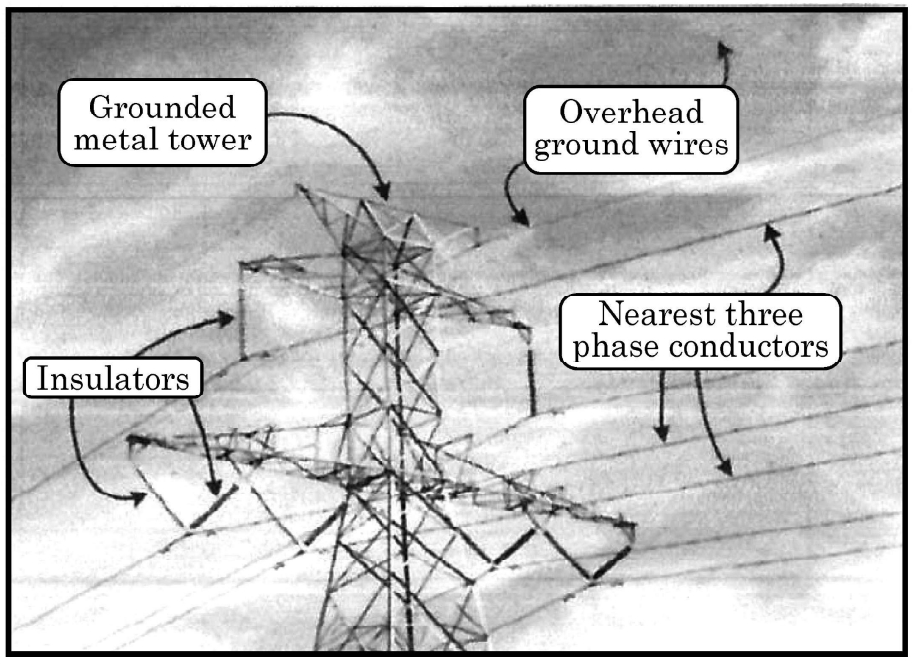
\includegraphics[width=\columnwidth]{txn}
			\caption{Electrical transmission wires connected to a transmission tower.}
			\label{fig:txn1}
		\end{figure}
		Two such wires in the figure \ref{fig:txn1} lie along the following lines:
		\begin{align}
			l_1 &: \dfrac{x+1}{3}=\dfrac{y-3}{-2}=\dfrac{z+2}{-1}\\
			l_2 &: \dfrac{x}{-1}=\dfrac{y-7}{3}=\dfrac{z+7}{-2}
		\end{align}
		Based on the given information, answer the following questions:
		\begin{enumerate}
			\item	Are the $l_1$ and $l_2$ coplanar? Justify your answer.
			\item    Find the point of intersection of lines $l_1$ and $l_2$.
		\end{enumerate}

	\item Write the cartesian equation of the line PQ passing through points P$(2,2,1)$ and Q$(5,1,-2)$. Hence, find the y-coordinate of the point on the line PQ whose z-coordinate is -2.

	\item Find the distance between the lines $x=\dfrac{y-1}{2}=\dfrac{z-2}{3}$ and $x+1=\dfrac{y+2}{2}=\dfrac{z-1}{3}$.
	
	\item Find the shortest distance between the following lines:
		\begin{align}
			\vec{r}&=3\hat{i}+5\hat{j}+7\hat{k}+\lambda(\hat{i}-2\hat{j}+\hat{k})\\\vec{r}&=(-\hat{i}-\hat{j}-\hat{k})+\mu(7\hat{i}-6\hat{j}+\hat{k})
		\end{align}

	\item Two motorcycles A and B are running at a speed more than the allowed speed on the road (as shown in figure \ref{fig:bike1}) represented by the following lines 
		\begin{align}
			\vec{r}&=\lambda(\hat{i}+2\hat{j}-\hat{k})\\\vec{r}&=(3\hat{i}+3\hat{j})+\mu(2\hat{i}+\hat{j}+\hat{k})
		\end{align}
		\begin{figure}[H]
			\centering
			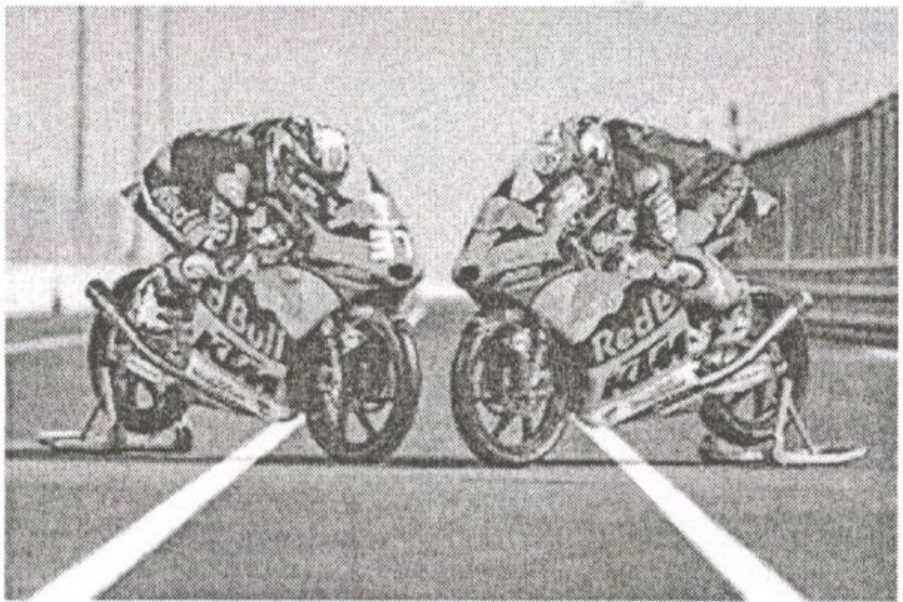
\includegraphics[width=\columnwidth]{bike}
			\caption{Two motorcycles moving along the road in a straight line.}
			\label{fig:bike1}
		\end{figure}
		Based on the following information, answer the following questions:
		\begin{enumerate}
			\item Find the shortest distance between the given lines.
			\item Find a point at which the motorcycles may collide.
		\end{enumerate}
	
	\item Find the shortest distance between the following lines
		\begin{align}
			\vec{r}&=(\lambda+1)\hat{i}+(\lambda+4)\hat{j}-(\lambda-3)\hat{k}\\\vec{r}&=(3-\mu)\hat{i}+(2\mu+2)\hat{j}+(\mu+6)\hat{k}
		\end{align}
	
	\item Find the shortest distance between the following lines and hence write whether the lines are intersecting or not.
		\begin{align}
			\dfrac{x-1}{2}=\dfrac{y+1}{3}=z, \dfrac{x+1}{5}=\dfrac{y-2}{1}, z=2
		\end{align}
\end{enumerate}
%\end{document}

\section{Perpendicular}
%\documentclass{exam}
%\usepackage{amsmath}
%\usepackage{enumitem}
%\begin{document}
\begin{enumerate}
\item If the distance of the point $(1,1,1)$ from the plane $x-y+z+\lambda=0$ is $\dfrac{5}{\sqrt{3}}$, find the value(s) of $\lambda$.
\item Find the distance of the point $(2,3,4)$ measured along the line $\dfrac{x-4}{3}=\dfrac{y+5}{6}=\dfrac{z+1}{2}$ from the plane $3x+2y+2z+5=0$.
\item Find the distance of the point $P(4,3,2)$ from the plane determined by the points $A(-1,6,-5),B(-5,-2,3)$ and $C(2,4,-5)$.
\item The distance of the line $\overrightarrow{\textbf{r}}=(\hat{i}-\hat{j})+\lambda(\hat{i}+5\hat{j}+\hat{k})$ from the plane $\overrightarrow{\textbf{r}}\cdot(\hat{i}-\hat{j}+4\hat{k})=5$ is
\begin{enumerate}
\item $\sqrt{2}$
\item $\dfrac{1}{\sqrt{2}}$
\item $\dfrac{1}{3\sqrt{2}}$
\item $\dfrac{-2}{3\sqrt{2}}$
\end{enumerate}
\item Find a unit vector perpendicular to each of the vectors $(\overrightarrow{a}+\overrightarrow{b})$ and $(\overrightarrow{a}-\overrightarrow{b})$ where $\overrightarrow{a}=\hat{i}+\hat{j}+\hat{k}$, $\overrightarrow{b}=\hat{i}+2\hat{j}+3\hat{k}$.
\end{enumerate}
%\end{document}


\section{Plane}
%\documentclass{exam}
%\usepackage{enumitem}
%\usepackage{amsmath}
%\begin{document}
\begin{enumerate}
\item Find the equation of the plane passing through the points $(2,1,0),(3,-2,-2)$ and $(1,1,7)$. Also, obtain its distance from the origin.
\vspace{4mm}
\item The foot of a perpendicular drawn from the point $(-2,-1,-3)$ on a plane is $(1,-3,3)$. Find the equation of the plane.
\vspace{4mm}
\item Find the cartesian and the vector equation of a plane which passes through the point $(3,2,0)$ and contains the line $\dfrac{x-3}{1}=\dfrac{y-6}{5}=\dfrac{z-4}{4}$.
\vspace{4mm}
\item The distance between the planes $4x-4y+2z+5=0$ and $2x-2y+z+6=0$ is
	\begin{itemize}
		\vspace{2mm}
	%	\renewcommand{\choicelabel}{(\thechoice)}
	\item $\dfrac{1}{6}$
	        \vspace{2mm}
	\item $\dfrac{7}{6}$
		\vspace{2mm}
	\item $\dfrac{11}{6}$
		\vspace{2mm}
	\item $\dfrac{16}{6}$
	\end{itemize}
		\vspace{4mm}
	\item Find the equation of the plane through the line of intersection of the planes $\overrightarrow{\textbf{r}}\cdot(\hat{i}+3\hat{j})+6=0$ and $\overrightarrow{\textbf{r}}\cdot(3\hat{i}-\hat{j}-4\hat{k})=0$, which is at a  unit distance from the origin.
\end{enumerate}
%\end{document}

\section{Miscellaneous }
%\documentclass{exam}
%\usepackage{float}
%\usepackage{array}
%\usepackage{enumitem}
%\usepackage{amsmath}
%\begin{document}
\begin{enumerate}
	\item Find the distance of the point $(1,-2,9)$ from the point of intersection of the line\\ 
		\begin{align*}
			\overrightarrow{\textbf{r}}=4\hat{i}+2\hat{j}+7\hat{k}+\lambda(3\hat{i}-+4\hat{j}+2\hat{k})
		\end{align*}and the plane 
		\begin{align*}
			\overrightarrow{\textbf{r}}\cdot(\hat{i}-\hat{j}+\hat{k})=10.
		\end{align*}
	\item Find the area bounded by the curves $y=\abs{x-1}$ and $y=1$, using integration.
\item Find the coordinates of the point where the line through $(4,-3,-4)$ and $(3,-2,2)$ crosses the plane $2x+y+z=6$.
\item Fit a straight line trend by the method of least squares and find the trend value for the year 2008 for the following data:
	\begin{table}[H]
		\input{table2}
	\end{table}
\end{enumerate}
%\end{document}

%\section{Exemplar}
%\input{exemplar/11.10.3}
%\section{Singular Value Decomposition}
%\input{svd/svd.tex}
%
%\chapter{Constructions}
%\section{JEE}
%\input{jee/7.tex}
%--------------------------------------------------------
%\section{Properties}
%\input{chapters/9/9/3.tex}
%
%\section{Properties}
%\input{chapters/9/8/1.tex}
%\section{Mid Point Theorem}
%\input{chapters/9/8/2.tex}
%\section{Parallelograms}
%\section{Triangles and Parallelograms}
%\input{chapters/9/9/4.tex}
%--------------------------------------------------------

%\chapter{Circles}
%
%\chapter{Tangents to a Circle}

\iffalse
\chapter{Conics}
\section{Circle}
\input{chapters/circles/examples/equation.tex}
\section{Exercises}
\input{chapters/circles/exer/equation.tex}
\section{Construction}
\input{chapters/circles/examples/const.tex}
\section{Exercises}
\input{chapters/circles/exer/const.tex}
\section{Parabola}
\input{chapters/conics/examples/parab.tex}
\section{Exercises}
\input{chapters/conics/exer/parab.tex}
\section{Ellipse}
\input{chapters/conics/examples/ellipse.tex}
\section{Exercises}
\input{chapters/conics/exer/ellipse.tex}
\section{Hyperbola}
\input{chapters/conics/examples/hyper.tex}
\section{Exercises}
\input{chapters/conics/exer/hyper.tex}

%
\fi


%\include{ch02} 
\backmatter
\appendix
\iffalse
\chapter{ Vectors}
\section{$2\times 1$ vectors}
\input{matrix/two.tex}
%\include{app01}
%\appendix
\section{$3\times 1$ vectors}
\input{matrix/three.tex}
\chapter{Matrices}
\input{matrix/mat.tex}
\input{linman/chapters/decomp/svd.tex}

\chapter{Triangle Constructions}
\input{cons/tri.tex}


\chapter{Linear Forms}
\section{Two Dimensions}
\input{linear/two.tex}
\section{Three Dimensions}
\input{linear/three.tex}
\chapter{Quadratic Forms}
%\numberwithin{equation}{subsection}
%\numberwithin{equation}{section}
\section{Conic equation }
\input{quad/defs.tex}
\section{Circles}
\input{quad/circle.tex}

\section{Standard Form}
\input{quad/stddef.tex}
\chapter{Conic Parameters}
\section{Standard Form}
\input{quad/standard.tex}
\section{Quadratic Form }
\input{quad/coroll.tex}

\chapter{Conic Lines}
\section{Pair of Straight Lines}
%
\input{quad/pair.tex}
\section{Intersection of Conics}
\input{quadlines/inter.tex}
\section{ Chords of a Conic}
\input{quadlines/chord.tex}
\section{ Tangent and Normal}
\input{quadlines/tangent.tex}
\fi
%\chapter{Proofs}
%   \section{}
%\input{apps/defs.tex}

%  \section{}
%\input{apps/parab.tex}
%  \section{}
%\input{apps/nonparab.tex}
%		\section{}
%\input{apps/params.tex}
\latexprintindex

\end{document}

 
\section{Examples}
\subsection{Loney}
\input{examples/loney.tex}
\subsection{Miscellaneous}
%\documentclass{exam}
%\usepackage{float}
%\usepackage{array}
%\usepackage{enumitem}
%\usepackage{amsmath}
%\begin{document}
\begin{enumerate}
	\item Find the distance of the point $(1,-2,9)$ from the point of intersection of the line\\ 
		\begin{align*}
			\overrightarrow{\textbf{r}}=4\hat{i}+2\hat{j}+7\hat{k}+\lambda(3\hat{i}-+4\hat{j}+2\hat{k})
		\end{align*}and the plane 
		\begin{align*}
			\overrightarrow{\textbf{r}}\cdot(\hat{i}-\hat{j}+\hat{k})=10.
		\end{align*}
	\item Find the area bounded by the curves $y=\abs{x-1}$ and $y=1$, using integration.
\item Find the coordinates of the point where the line through $(4,-3,-4)$ and $(3,-2,2)$ crosses the plane $2x+y+z=6$.
\item Fit a straight line trend by the method of least squares and find the trend value for the year 2008 for the following data:
	\begin{table}[H]
		\input{table2}
	\end{table}
\end{enumerate}
%\end{document}

%
%%\section*{Disclosure Statement}
%%The authors report there are no competing interests to declare.
%%
%%
%%
%%  
%%%All the results related to conics are summarized in 
%%%Table \ref{table:conics}.  
%%%\begin{table*}[!t]
%%%\centering
%%%\input{conics.tex}
%%%%\input{./figs/conics.tex}
%%%\caption{$\vec{x}^{\top}\vec{V}\vec{x}+2\vec{u}^{\top}\vec{x}+f = 0$  can be expressed in the above standard form for various conics. $\vec{c}$ represents the centre/vertex of the conic. $\vec{q}$ is/are the point(s) of contact for the tangent(s). }
%%%\label{table:conics}
%%%\end{table*}
%%%\begin{verbatim}
%%\bibliographystyle{tfs}
%%%\bibliography{interacttfssample}
%%\bibliography{school}
%%\end{verbatim}
%% included where the list of references is to appear, where \texttt{tfs.bst} is the name of the \textsc{Bib}\TeX\ bibliography style file for Taylor \& Francis' Reference Style S and \texttt{interacttfssample.bib} is the bibliographic database included with the \textsf{Interact}-TFS \LaTeX\ bundle (to be replaced with the name of your own .bib file). \LaTeX/\textsc{Bib}\TeX\ will extract from your .bib file only those references that are cited in your .tex file and list them in the References section.
%
%% Please include a copy of your .bib file and/or the final generated .bbl file among your source files if your .tex file does not contain a reference list in a \texttt{thebibliography} environment.
%

  % \section{Appendices}
  % \appendix
			\appendices
